\label{chapter:rts_ratio}

% methodology

% 3.	Faculty Workload Allocation Model (R >T <S)
% 4.	Modelling Research Workload (Relative (not absolute) Association) – in progress
% 5.	Modelling Teaching Workload (classification based on formal/informal teaching) – already uderway
%	 5.1.	Formal teaching – max cap to limit the formal teaching workload among Lect/Profs
%	 5.2.	Informal teaching workload – zero sum game
Due to the various activities that faculty are involved in, and their varying degrees of involvement, distributing the teaching workload equally between the faculty would lead to an unequal overall workload. Thus, modelling faculty workload is an important activity in maintaining equity in the teaching workload distribution. This section delves into the workload allocation model used for distributing the teaching workload.

\section{Workload Allocation Model (WAM)}
The inclusion of research and service/administrative workloads along with teaching workload has previously led to admirable results in existing Workload Allocation Models (WAMs) like \parencite{finlay1994management} and \parencite{griffith2020framework}. \parencite{rohan2017} demonstrated how, in a teaching allocation-centric view, research and service workloads can be used to offset the teaching workload by giving relaxations for the same. However, to give a transparent and comprehensive view of a faculty's workload, we chose to give a clear picture of all three aspects of the faculty's workload.

We define the total workload \(W_f\) of a faculty \(f\) as constituted by 3 parts \(R_f + T_f + S_f\) for Teaching, Research and Service respectively. Since, the aim is to distribute an equal amount of workload to all faculties, we thus choose an equal total workload \(W\) for all faculty. After fitting for the units described in later sections, we chose the value \(W = 12\). Thus,
\[W_f = R_f + T_f + S_f = 12\]
\section{Workload Allocation Model principles}

\parencite{trac2011} lists the principles that guide WAMs:

\begin{enumerate}
    \item \textbf{Equity}

          \begin{itemize}
              \item{Inclusive of all academic, teaching, and research staff}
              \item{Form a neutral framework with the ability to adopt local variable factors}
              \item{Quantifies All activities}
          \end{itemize}
    \item \textbf{Transparency}
          \begin{itemize}
              \item{Clear and understandable}
              \item{Consistent application}
              \item{Enable appropriate “visibility” of staff activities}
          \end{itemize}
    \item \textbf{Consultation}
          \begin{itemize}
              \item{Ongoing process open to development and improvement}
          \end{itemize}
\end{enumerate}

Faculty members in universities commonly perceive their own teaching workload as higher than average, and their own department’s workload assignment as unfair \parencite{2018exploring}. Thus, a transparent workload model is important for staff satisfaction. Also, the accuracy of the model depends on its ability to closely describe and encapsulate all the work of a faculty, while its utility lies in the ability to abstract said work into broad areas for transparency and analytical purposes. \parencite{vardi2009impacts} describes this push and pull between accuracy and simplicity, and that WAM complexity is known to cause dissatisfaction.

Existing workload models operate on various ideologies for quantifying the amount or value of work delivered by a faculty. A common ideology is to quantify work on the basis of the amount of time spent. One such ideology is using measurable outputs to quantify the value of work done by individual faculty. In the case of teaching output, this could be the total academic credits students have acquired \parencite{trac2011}

\section{Modelling Research Workload}
As previously mentioned, research supervision workload i.e. the amount of work spent in the supervision of research staff (Post-Docs and Research Assistants/Associates) \parencite{rohan2017} makes for a useful proxy to measure the overall research workload. However, the aim of the WAM is to define the total workload accurately. Thus, we account for the scholarly research work (research work, publishing papers etc) by splitting \(R_f\) into two parts.
\[R_f = R^b_f + R^s_f\]
\(R^b_f\) is the Scholarly Workload for the faculty, defined by faculty type. \(R^s_f\) is amount of Supervision Workload defined by the amount of work required for managing aforementioned research staff.
\subsubsection{Hierarchy effects in Research Supervision Workload}
\begin{figure}[H]
    \centering
    \scalebox{.5}{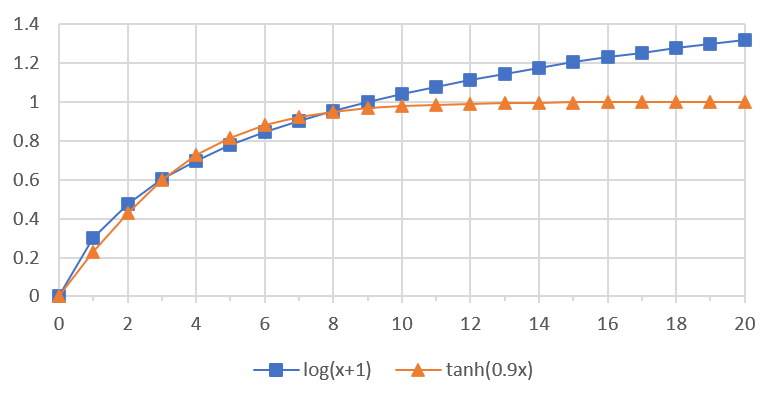
\includegraphics{images/plot_tanh_log.png}}
    \caption{Plot of tanh and log functions}
    \label{fig:plot_tanh_log}
\end{figure}
However, it fails to account for hierarchy effects and economies-of-scale where, as the research staff members increase, they self-organize into a hierarchy, thus reducing the supervision workload on the faculty \parencite{WANG2015197,wellman1997electronic}. We aim to account for this using some non-linearity in the supervision workload. We currently use \(tanh\) due to its closeness to logarithmic functions which tapers off to a maximum (\autoref{fig:plot_tanh_log}), however, more testing is required to arrive at the final definition of the supervision workload, including the weights of research staff types.

\begin{equation}
    \begin{aligned}
        R^s_f & = r\bigg[\frac{2}{(1 + s^{-w} )}- 1\bigg] \\
        w     & = \sum_{r \epsilon R} w_r * n_r           \\
    \end{aligned}
\end{equation}
where,
\begin{equation}
    \nonumber
    \begin{aligned}
        w   & = \text{Sum of total research staff weights} \\
        w_r & = \text{Weight of individual staff type }r   \\
        n_r & = \text{Total number of staff of type }r     \\
        R   & = \text{Set of all staff types}              \\
    \end{aligned}
\end{equation}
\begin{table}[H]
    \centering
    \begin{tabular}{|l|c|c|}
        \hline
        Staff Type         & \(w_r\) \\
        \hline
        Research Assistant & 2       \\
        Post Doc           & 1       \\
        \hline
    \end{tabular}
    \caption{Weights of different research staff types}
\end{table}

Where, \(r\) and \(s\) are parameters defined by the faculty type, to control the behaviour of the function. As an example, for full time professors, we could arrive at \(r=2, s=1.32, R_b = 6 \), thus arriving at the equation below. \autoref{fig:teaching_workload} the plot of the total research workload, for such a distribution  approximated to the nearest \(0.25\) units to make it more realizable.

\[R_f = 6 + 2\bigg[\frac{2}{(1 + 1.32^{-w} )}- 1\bigg]\]

\begin{figure}[H]
    \centering
    \scalebox{0.4}{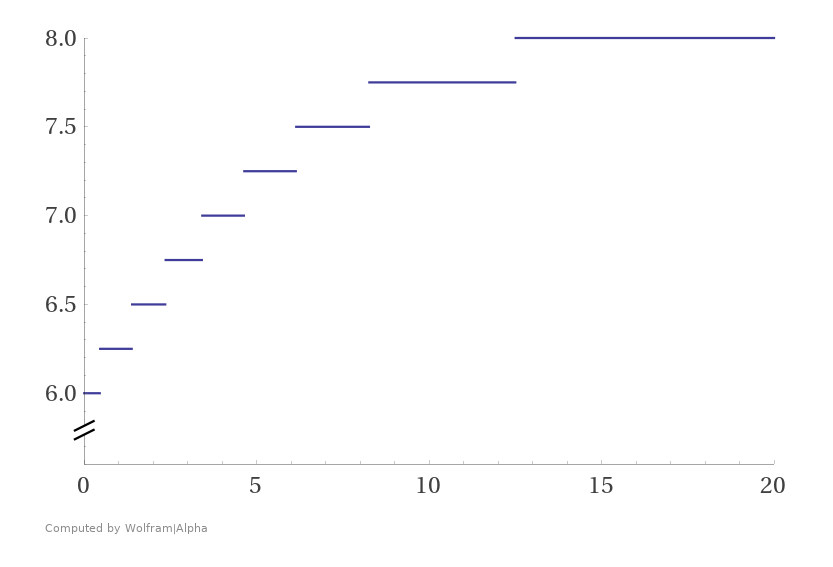
\includegraphics{images/Teaching workload.png}}
    \caption{Teaching Workload}
    \label{fig:teaching_workload}
\end{figure}
\section{Modelling Service Workload}
Service is a challenging part of the workload to measure due to its lack of objectively measurable outputs. In this work, the approach towards quantifying the service workload involves a points system where every service duty \(d\) (like industry attachment officer, course allocation coordinator) corresponds to a set weight \(w_d\). The weighted sum of all the service points will then be normalized to get the service duty workload \(S^d_f\). Similar to the research workload, there will also be a baseline service workload \(S^b_f\) involved to account for faculty-type based service duties (like peer reviews).
\begin{equation}
    \begin{aligned}
        S_f   & = S^b_f + S^d_f                      \\
        S^d_f & = n *\sum_{d\epsilon D}  (w_d * d_f)
    \end{aligned}
\end{equation}
where,
\begin{equation}
    \nonumber
    \begin{aligned}
        w_d & = \text{Weight of the individual service duty }d                    \\
        d_f & = 1\text{, if faculty f carries duty }d\text{, else }0              \\
        n   & = \text{Normalization factor to convert weights into service ratio} \\
        D   & = \text{Set of all service duties}
    \end{aligned}
\end{equation}


However, further exploration is required to list for all the service responsibilities and their corresponding weights. There's also some danger that some service duties cannot be accounted for in this manner, or that certain duties might have different weights faculty to faculty.

\section{Modelling Teaching Workload}
\label{teaching_workload}

Since for a faculty \(f\), the Total Workload \(W_f\) remains fixed, the teaching workload \(T_f\) can be calculated right after the service and research workload has been defined.
\begin{equation}
    \begin{aligned}
        T_f & = W_f - (R_f + S_f)                      \\
        T_f & = 12 - (R^b_f + R^s_f) - (S^b_f + S^d_f)
    \end{aligned}
\end{equation}
As a point of reference and comparison, we define \(T_b\) as the base teaching value for a faculty with no extra Research Supervision and Service Duty workload,  \(R^s_f = S^d_f = 0\). Or simply, \(T^b_f = 12 - R^b_f - S^b_f\). As a shorthand, the ratio of \(R^b_f : T^b_f  : S^b_f\)  for a faculty type will be referred to as the \textbf{RTS ratio}.

\begin{table}[h]
    \centering
    \begin{tabular} { |l |c |c|c|}
        \hline
                  & \(R\) & \(T\) & \(S\) \\
        \hline
        Lecturer  & 2     & 8     & 2     \\
        Professor & 6     & 4     & 2     \\
        \hline
    \end{tabular}
    \caption{RTS Ratio for different faculty types}
    \label{rts_ratio}
\end{table}

Since the total amount of teaching workload (total number of courses taught) remains constant, this teaching ratio is used to calculate the distribution of the fixed teaching workload among all the faculty.
